\chapter{Desarrollo de Aplicaciones}

Una vez explicadas todas las tecnologías y expuestos los objetivos de este trabajo, se dará utilidad a todos estas herramientas. Para ello se han creado dos aplicaciones. La primera SurveillanceApp, se trata de una aplicación web capaz de manejar eventos en YouTube. La segunda consiste en usar las herramientas de JdeRobot para capturar el flujo de vídeo y retransmitirlo a través de YouTube.

\section{SurveillanceApp}

Como se ha comentado anteriormente el objetivo de esta aplicación es poder manejar eventos programados en YouTube y retransmitir el contenido capturado por un elemento hardware que en nuestro caso será una cama web. La aplicación incorpora las siguientes funcionalidades.

\begin{enumerate}
    \item Permite crear eventos programados y asociados a un canal de YouTube
    \item Permite iniciar y detener la retransmisión del evento a través de ffmpeg
    \item Permite añadir subtítulos al evento retransmitido.
    \item Muestra en su pantalla principal los eventos en directo asociados a un canal de YouTube.

\end{enumerate}

Antes de pasar a analizar el código se explicara la arquitectura con el objetivo de entender mejor su funcionamiento.
La aplicación usa un servidor programado en nodeJS, dicho servidor es el encargado de recoger los datos e instrucciones dados por el usuario a través de la interfaz web y comunicárselo a los scripts desarrollados con las librerías de YouTube API. Dichos scripts se encuentran desarrollados en Python.
Para la ejecución de los scripts de Python se ha utilizado child process, un módulo de nodeJS capaz de ejecutar comandos en la terminal de esta forma podemos comunicarnos con Youtube.
El flujo audiovisual es recogido a través de ffmpeg mediante la herramienta video4linux2 , que se encarga de recoger el contenido capturado vía hardware por una cámara web con micrófono incorporado. Para la ejecución de ffmpeg se sigue la misma técnica que con los scripts de YouTube. También es ffmpeg quien se encarga de retransmitir el flujo hacia los servidores de YouTube.
Cabe destacar que la aplicación implementa una seguridad adicional a la de YouTube. Esto se debe a que en la aplicación se manejan datos privados relacionados con la cuenta de Google del usuario, por ello se ha implementado un mecanismo de seguridad basado en un middleware y el establecimiento de sesión. El middleware es un mecanismo que protege ciertas rutas de acceso, por ejemplo si queremos acceder a la parte de creación de eventos el middleware servirá un formulario de identificación. Una vez identificado se crea una sesión de usuario para no identificarnos continuamente.

\begin{figure}[H]
    \centering
    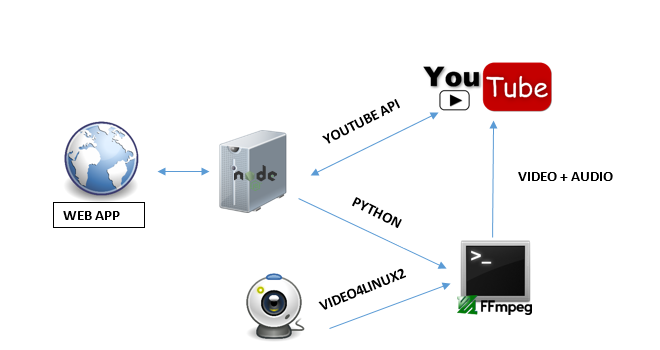
\includegraphics[width=150mm]{surveillance-arquitectura.PNG}
    \caption{Arquitectura SurveillanceApp}
\end{figure}

\subsection{Comunicación con Python}

Una de las dificultades encontradas a la hora de desarrollar la aplicación es que las librerías proporcionadas por YouTube no presentan una versión estable para JavaScript. Como se ha comentado anteriormente las funcionalidades relacionadas con YouTube han sido desarrolladas con Python, como se podrá ver más adelante. 
Para manejar estos scripts se ha recurrido al módulo child\_process, que forma parte de NodeJS. A través de este módulo Node nos proporciona la opción de crear un proceso hijo de forma asíncrona, es decir sin bloquear el flujo principal del servidor. Child\_proccess proporciona varios métodos para realizar esta tarea, en esta aplicación se usara el método spawn, que es capaz de generar un nuevo proceso a partir de un comando dado, en nuestro caso el comando será el de ejecución de ficheros Python.
El método toma tres argumentos \textbf{child\_process.spawn(command[, args][, options])} , el primero es el comando a ejecutar, el segundo un array con los argumentos del comando si este los tuviera y por ultimo opciones del comando. De esta forma se crea un proceso paralelo al servidor capaz que ejecuta el comando en un terminal del sistema sin bloquear al servidor.
A continuación se incluye un fragmento de código donde se puede ver el uso del módulo dentro de la aplicación. En el podemos observar una primera sentencia donde se crea el proceso haciendo uso de spawn , ejecutando el script de Python. Una vez generado el proceso este proporciona dos salidas stdout y stderr.

\begin{itemize}
    \item \textbf{stdout}, recoge los datos devueltos por Python. De esta forma si desde Python queremos enviar datos al flujo principal debemos hacerlo mediante el método print y serán recogidos por stdout.
    \item \textbf{stderr}, aquí se recoge la salida de error tanto para errores de ejecución del comando como errores que puedan surgir dentro del script.
\end{itemize}

\begin{lstlisting}[language = JavaScript] 

exports.retrieveStreamList =  function(req,res,status){

    var process = spawn('python',['./public/python/streamList.py', ' --status' , status]);
    processOutput(res,process);
}

function processOutput(res,process){

    var py_data;
    var py_err;
    
    process.stdout.on("data",function(data){
            py_data += data; 
    })
    
    process.stdout.on("end",function(){

    if(typeof py_data !== "undefined"){
      py_data = py_data.substring(9);
      console.log(py_data)
      if(py_data.localeCompare("ERROR") == 1){
        res.status(500).end();
      }else{
          res.end(py_data)
      }
        }   
    })

    process.stderr.on("data", function(data){
        py_err += data;
    })
    process.stderr.on("end",function(){
    
        if(typeof py_err !== 'undefined'){
            res.status(500).end()
            console.log("Python Error: " + py_err)
        }   
    })
}

\end{lstlisting}

\subsection{Comunicación con YouTube}

Como ya sabemos para esta comunicación se han usado las librerías proporcionadas por YouTube API. YouTube API proporciona muchas alternativas, para esta aplicación se han elegido dos recursos livebroadcast y livestream ambos explicados en el capítulo tres. Con estos recursos hemos desarrollado tres funcionalidades relacionadas con YouTube en la aplicación, separadas en tres scripts de Python. Todas ellas tienen en común la parte de autenticación que implementa  el protocolo OAuth 2.0.

\\

\begin{lstlisting}[language=Python]

    # The CLIENT_SECRETS_FILE variable specifies the name of a file that contains
    # the OAuth 2.0 information for this application, including its client_id and
    # client_secret.
    
    CLIENT_SECRETS_FILE = "./private/client_secret.json"
    
    YOUTUBE_READ_WRITE_SCOPE = "https://www.googleapis.com/auth/youtube"
    YOUTUBE_API_SERVICE_NAME = "youtube"
    YOUTUBE_API_VERSION = "v3"
    
    MISSING_CLIENT_SECRETS_MESSAGE = """
    WARNING: Please configure OAuth 2.0
      
    """
    def get_authenticated_service(args):
    
      flow = flow_from_clientsecrets(CLIENT_SECRETS_FILE,
        scope=YOUTUBE_READ_WRITE_SCOPE,
        message=MISSING_CLIENT_SECRETS_MESSAGE)
    
      storage = Storage("%s-oauth2.json" % sys.argv[0])
      credentials = storage.get()
    
      if credentials is None or credentials.invalid:
        credentials = run_flow(flow, storage, args)


\end{lstlisting}

En este fragmento de código aparecen varias cosas importantes para poder entender el funcionamiento de las librerías. Como se ha comentado en el capítulo tres YouTube ha adoptado Oauth 2.0 como sistema de autenticación. Para poder usar las librerías de YouTube primeramente debes registrarte en la consola de desarrolladores de Google  y dar de alta tu proyecto y una vez dado de alta debes habilitar las API que tu proyecto usara. Terminado este proceso obtendrás el secreto de cliente (clien\_secret.json), es un fichero el cual contiene las credenciales que te identifican como propietario de la cuenta de Google \footnote{https://console.developers.google.com} asociada al proyecto.

Otra parte importante es la de los ámbitos o scope. Esta parte especifica que permisos tiene para interactuar con YouTube la aplicación. Por ejemplo en el código escrito arriba el scope, permite tanto leer como modificar los recursos asociados a la cuenta de YouTube. Los otros parámetros indican el API que va a ser usada y su versión. 

A continuación nos encontramos con el método que lleva a cabo el proceso de autenticación. Dicho método es proporcionado por Google en la documentación de la API. Este método busca un fichero con las credenciales que autorizan a la aplicación a acceder a los datos almacenados en la cuenta de YouTube asociada a la misma. Si es la primera vez que se accede estos datos no estarán generados por lo cual se redirigirá automáticamente al usuario a los servidores de autenticación de Google. Si la autenticación ha sido correcta se creara automáticamente un fichero que permite el acceso a la cuenta por parte de la aplicación.

\begin{itemize}
    \item \textbf{Creación de eventos}
    
    Una de las funcionalidades que nos permite la aplicación es la creación de eventos programados. Para ellos a través de un formulario contenido en la interfaz web son recogidos una serie de datos como el título del evento, el horario, la privacidad o la calidad del mismo, todas ellas propiedades de ambos recursos. Estos datos son enviados al servidor en formato JSON y proporcionados como entrada a createEvent.py.  CreateEvent hace uso del método insert tanto de livebroadcast como de livestream para crear ambos recursos. Una vez creados se recupera su ID para proporcionárselo al método bind perteneciente a livebroadcast de forma que el evento es creado en el canal asociado.
\\  
    \begin{lstlisting}[language=Python]
    # Create a liveBroadcast resource and set configuration
    def insert_broadcast(youtube, options):
      insert_broadcast_response = youtube.liveBroadcasts().insert(
       part="snippet,status,contentDetails",
        body=dict(snippet=dict(
            title= args["broadcast_title"],
            scheduledStartTime= args["start_time"]),
    
          status=dict(
            privacyStatus= args["privacy"]),
          contentDetails=dict(
            monitorStream=dict(
              enableMonitorStream = 'true')
            )  
    )
      ).execute()

    snippet = insert_broadcast_response["snippet"]
    return insert_broadcast_response["id"]

    # Create a liveStream resource and set configuration
    def insert_stream(youtube, options):
        insert_stream_response = youtube.liveStreams().insert(
            part="snippet,cdn",
            body=dict(
                snippet=dict(
                    title= args["broadcast_title"]
                ),
                cdn=dict(
                    format= args["format"],
                    ingestionType="rtmp"
                )
             )
        ).execute()

    snippet = insert_stream_response["snippet"]
    return insert_stream_response["id"]

    # Bind the broadcast to the video stream.
    def bind_broadcast(youtube, broadcast_id, stream_id):
        bind_broadcast_response = youtube.liveBroadcasts().bind(
        part="id,contentDetails",
        id=broadcast_id,
        streamId=stream_id
        ).execute()
    \end{lstlisting}
    
    \item \textbf{Recuperación de información}
    
    Dentro de la aplicación en su pantalla principal podemos ver el vídeo de aquellos eventos que se encuentran en directo sin necesidad de acudir a YouTube, esto es posible gracias a que YouTube mediante su propiedad monitorStream nos proporciona un i-frame el cual tiene como fuente(source) un reproductor de YouTube embebido asociado al nuestro evento. Por otro lado dentro de la parte privada de la aplicación, únicamente accesible para administradores, se pueden ver los eventos programados e iniciar su retransmisión o los eventos que se están retransmitiendo para detenerlos.
    Todas estas funcionalidades requieren de datos proporcionados por los servidores de YouTube, para recuperar estos datos se recurre al método list, perteneciente tanto al recurso livebroadcast como al livestream. Dicho método admite filtros para buscar los eventos que nos interesan, en nuestro caso filtramos por el estado del evento, activo o programado, y además especificamos las partes del recurso que queremos recuperar  por último se limitan los resultados a 50.
    
    \begin{lstlisting}[language =Python]
    
    list_broadcasts_request = youtube.liveBroadcasts().list(
        broadcastStatus= status,
        part="snippet, contentDetails",
        maxResults=50
          )
    \end{lstlisting}

    En el caso de livestream recuperamos únicamente el stream asociado a la retransmisión mediante su ID, de este recurso nos interesa su propiedad cdn ya que de ahí obtenemos el stream\_name, necesario para la posterior retransmisión ya que este ID identifica al recurso \footnote{Capítulo 3. Propiedades livestream y livebroadcast} en los servidores de ingestión de contenido de YouTube, además recuperamos los datos de ingestión como la calidad del evento de forma que luego se pueden calcular datos como bitrate o resolución. Otras propiedades importantes que recuperamos son monitor que contiene un iframe que posteriormente se inserta en la aplicación web para poder visualizar el evento una vez activo.
    Una vez recuperados son almacenados en list\_broadcast\_request. Este objeto contiene la información de todos los eventos y de él recuperamos la información que nos interesa de cada uno y formamos un JSON que será la respuesta a la petición web.
    \\


    \begin{lstlisting}[language =Python]
    
    while list_broadcasts_request:
        broadcast_response = list_broadcasts_request.execute()
        for broadcast in broadcast_response.get("items", []):
    
        title = broadcast["snippet"]["title"]
        monitorStream = broadcast["contentDetails"]["monitorStream"]["embedHtml"]
        stream_id = broadcast["contentDetails"]["boundStreamId"]
        cdn = getStreamKey(youtube,stream_id)
        data_output["data"].append({"title" : title , "streamkey" : cdn["ingestionInfo"]["streamName"],
        "monitor": monitorStream, "quality" : cdn["format"],"broadcastID": broadcast["id"] })

        list_broadcasts_request = youtube.liveBroadcasts().list_next(list_broadcasts_request, broadcast_response)
    
    # Retrieve a livestream resource match with stream_id
    def getStreamKey(youtube,stream_id):
    
        list_streams_request = youtube.liveStreams().list(
        part="cdn",
        id=stream_id,
        maxResults=1
        )
        list_streams_response = list_streams_request.execute()
        return list_streams_response["items"][0]["cdn"]

    
    \end{lstlisting}
    
    \item \textbf{Terminar la retransmisión del evento}
    
    Esta es la última funcionalidad que le se le ha dado a la aplicación apoyándonos en la las librerías de YouTube. Para conseguir este objetivo se ha usado el método transition perteneciente al recurso livebroadcast. Con dicho método recuperamos una emisión en directo a partir de su ID y modificamos su estado de activo a finalizado, de esta forma YouTube dará por terminada la retransmisión y el evento finalizará. Tambien debemos acabar con la ejecución de ffmpeg ya que mientras este se este ejecutando no podremos iniciar la retransmisión de un nuevo evento ya que la camara estara ocupada por ffmpeg , para ello usamos el comanado -pkill ffmpeg, el cual acabar con el proceso.
    \\
    
    \begin{lstlisting}[language = Python]
    
    def stop_broadcast(youtube,brID):
        broadcast_request = youtube.liveBroadcasts().transition(
        broadcastStatus= "complete",
        id = brID,
        part = "status")
        broadcast_request.execute()
    
    \end{lstlisting}
    
    
    \item \textbf{Comunicación con ffmpeg}
    
    Ffmpeg es el encargado de enviar el flujo audiovisual a los servidores de ingestión de contenido de YouTube. Ffmpeg presenta varias herramientas pero para este objetivo únicamente hemos usado la funcionalidad que permite manejarlo desde la terminal. Para ello se ha desarrollado un script de Python que escribe en un fichero .sh el comando de ffmpeg a ejecutar, tras esto mediante la instrucción os.system se ejecuta el fichero. Para la construcción del comando ffmpeg se toma como entrada primeramente la calidad del evento, en función de esta calidad se añade el bitrate y la resolución del video según las especificaciones de YouTube. Otro parámetro fundamental que recibe el script es el stream\_key, representa un identificador único del stream dentro de los servidores de YouTube para que este pueda asociar el flujo audiovisual recibido al evento.
    
    \begin{lstlisting}[language = Python]

    def list_streams(stream_key,resolution,bitrate):

    os.system("chmod +rw ./public/static/ffmpeg.sh")
    outfile = open('./public/static/ffmpeg.sh', 'w') 
    outfile.write('ffmpeg -f alsa -ac 2 -i default -f video4linux2’+ ‘-framerate 15 -video_size ' + resolution +
    '-i dev/video0 -vcodec libx264 -preset veryfast -minrate ' + bitrate  + '-maxrate 1000k -bufsize 1000k' +' -vf "format=yuv420p"  -g  30 ' + '-vf drawtext= "fontfile=/usr/share/fonts/truetype/freefont/FreeSerif.ttf:’+ ‘fontsize=24:''fontcolor=yellow:textfile=./public/static/subtitles.txt:reload=1 :x=100:y=50"' +
    ' -c:a libmp3lame -b:a 128k -ar 44100' +
    ' -force_key_frames 0:00:04 –f flv rtmp://a.rtmp.youtube.com/live2/' + Stream_key                 
    outfile.close()
    os.system("chmod 0755 ./public/static/ffmpeg.sh")
    os.system("./public/static/ffmpeg.sh")
    
    \end{lstlisting}
    
    Ffmpeg presenta una gran variedad de posibilidades a continuación se explican las principales partes del comando usado en el script:
    
    \begin{itemize}
        \item \textbf{Video4Linux y ALSA}, son componentes pertenecientes al SO Linux que se encargan de recoger los flujos de video y audio respectivamente. Como fuente de video usamos la cámara principal del sistema, /dev/video0, para el audio el micro definido por defecto.
        
        \item \textbf{Libx264}, códec de vídeo H264, tras el aparecen las opciones de codificación del video, el perfil no está especificado pero por defecto ffmepg usa el perfil básico del códec.
        
        \item \textbf{Drawtext}, opción usada para superponer texto sobre el vídeo, es la equivalencia a los subtítulos. El texto es leído de un fichero .txt, que tiene asociada la opción reload encargada de detectar el cambio en el fichero de texto. Las otras opciones lo acompañan se refieren al formato del texto mostrado en pantalla.
    
        \item \textbf{Force\_key\_frames}, a la hora de codificar el video se usan frames de referencia a partir de los cuales se codifican los siguientes, este comando obliga a enviar estos frames cada cuatro segundos.
        
        \item \textbf{Rtmp}, protocolo de comunicación usado entre el servidor de YouTube y ffmpeg para el intercambio del contenido.
    \end{itemize}
\end{itemize}


\section{Adaptador Ffmpeg para JdeRobot}

En esta segunda aplicación abordaremos la segunda parte del proyecto, hacer compatibles las herramientas de JdeRobot con los eventos en directo de YouTube, con el objetivo de retransmitir en directo el contenido captado por un UAV.Para conseguir este objetivo se ha desarrollado un "adaptador" capaz de unir JdeRobot con Ffmpeg para que este posteriormente retransmita el contenido a Youtube.

Ffmpeg presenta una opción con la cual usando como fuente de entrada una o varias imágenes ffmpeg es capaz de retornar un vídeo. En este caso solo hemos necesitado una imagen sobre la cual aplicamos un bucle infinito con el objetivo de que ffmpeg la use como fuente. Para entender mejor este proceso se muestra un ejemplo de comando que consigue este propósito.

\begin{lstlisting}[language=Python]

ffmpeg -loop 1 -i image.jpg -v:c libx264 -pix\_fmt yuv420p output.mp4

\end{lstlisting}

Como podemos ver mediante la opción -loop 1 se establece el bucle infinito comentado anteriormente que toma como entrada una imagen, de forma que si esta imagen varía con una frecuencia suficiente se obtendrá un vídeo fluido.

Una vez solucionado ffmpeg, el siguiente paso es encontrar una herramienta de JdeRobot capaz de proporcionar imágenes con una frecuencia suficiente como para poder crear un flujo de vídeo. Para ello se ha usado el componente cameraserver, explicado en el capitulo anterior. Dicho componente capta imágenes a una velocidad de unos 25 fps, suficiente para nuestro propósito. Dicho componente esta desarrollado en C++, pero presenta también un desarrollo en python que es el usado en este proyecto. 

Una vez encontrado el componente la idea general es enviar las imágenes capturadas en un UAV a un ordenador local a través de cameraserver, una vez en nuestro ordenador estas imágenes deben ser almacenadas localmente en un solo archivo, de forma que cada vez que una imagen nueva llegue al ordenador la antigua sea sobrescrita y finalmente ffmpeg acceda a esta imagen "dinámica" para formar el flujo de vídeo final.

\begin{figure}[H]
    \centering
    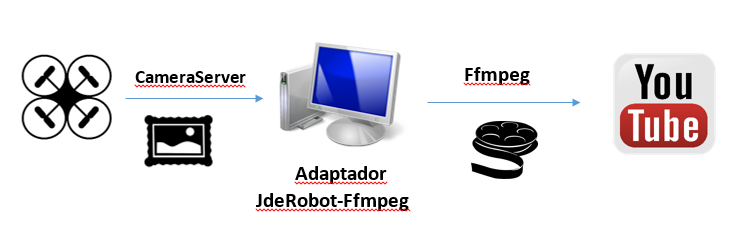
\includegraphics[width=150mm]{adapter.png}
    \caption{Esquema adaptador JdeRobot a ffmpeg}
\end{figure}

\subsection{Conexión mediante ICE}

Como se ha comentado anteriormente JdeRobot incluye distintos componentes que usan ICE para conectarse entre ellos. Para facilitar la conexión ICE en Python, JdeRobot ha desarrollado una serie de librerías que facilitan este proceso. Dentro de este proyecto se hace uso de easyiceconfig\_py \footnote{https://github.com/JdeRobot/JdeRobot/tree/master/src/libs/easyiceconfig_py} y parallelIce\_py \footnote{https://github.com/JdeRobot/JdeRobot/tree/master/src/libs/parallelIce_py}. El primero de ellos easyiceconfig es el encargado de obtener los parametros necessarios para inicializa la conexión para ellos usa la librerías de ICE pertenecientes a ZeroC.
Por otro lado tenemeos parallelICE que consiste en un conjunto de scripts que facilitan la conexión con los interfaces del dron (CameraClient, cmdvel, navDataClient,pose3D). Para nuestro objetivo únicamente necesitaremos conectarnos con la cámara por lo que usaremos cameraClient.py. Este script tiene implementada dos clases camera y cameraClient. La función de cameraClient es crear un hilo de ejecución que inicializa un objeto de clase camera, dicho objeto debe recibir como parámetros la conexión ICE inicializada previamente y por otro lado el nombre del interfaz, con estos datos se establece la conexión con la cámara del dron. Además de esto la clase camera tiene implementados métodos que nos devuelven tanto las imágenes del dron como información acerca de ellas, por lo que una vez instaciado el objeto simplemente deberemos llamar a su método getImage. Una vez entendidas las conexiones y las librerías usadas se muestra el desarrollo del código.



\subsection{Desarrollo}

Como base para desarrollar este adaptador se ha usado un proyecto perteneciente a JdeRobot color filter\footnote{http://jderobot.org/Teaching_robotics_with_JdeRobot#Color\_filter}, dicho proyecto esta desarrollado en python y permite aplicar filtros a las imágenes recogidas por un ordenador local procedentes de cameraserver.
Como ya hemos comentado anteriormente para realizar la comunicación entre el ordenador local, donde ejecutamos el adaptador, y cameraserver se usara una conexión ICE haciendo uso de las librerías desarrolladas por JdeRobot easyiceconfig y parallelICE. 
\\

\begin{lstlisting}[language=Python]

import sys
import easyiceconfig as EasyIce
from gui.threadGUI import ThreadGUI
from parallelIce.cameraClient import CameraClient
from gui.cameraWidget import CameraWidget
from PyQt5.QtWidgets import QApplication

if __name__ == '__main__':
    ic = EasyIce.initialize(sys.argv)
    prop = ic.getProperties()
    remoteCamera = CameraClient(ic, "Introrob.Camera", True)
    app = QApplication(sys.argv)
    camera = CameraWidget()
    camera.setCamera(remoteCamera)
    if (len(sys.argv)== 3 and sys.argv[2] == "GUI"):
        camera.setGUI = True
        camera.initUI()
        camera.show()
    else:
        print("For see the GUI, add to command GUI")


\end{lstlisting}

Los datos usados para esta conexión son recuperados de un fichero de configuración en el que se especifican la dirección y puerto en la que se esta ejecutando cameraserver.
\\
\begin{lstlisting}
Introrob.Camera.Proxy  = cameraA:default -h localhost -p 9999
\end{lstlisting}


Aprovechando la funcionalidad implementada de obtención de imágenes de cameraserver se ha creado el adaptador. Para solucionar el almacenaje de las imágenes en un ordenador local se ha usado la librería PIL de Python, esta librería se encarga del procesado de imágenes en Python. Cameraserver devuelve las imágenes en formato RGB y llegan al ordenador local como un array de datos, dicho formato es incompatible con ffmpeg por lo que a través del modulo image perteneciente a la librería PIL se transforma dicho array en una imagen, para ser posteriormente almacenada localmente en formato JPG, compatible con ffmpeg.
En este punto nos encontramos con un problema y es que los procesos del adaptador y de ffmpeg no están sincronizados, es decir a la vez que ffmpeg lee la imagen el adaptador esta escribiendo en ella por lo cual se produce un error. Para este error se proporcionan dos soluciones

\begin{itemize}
    \item La primera solución implica sustituir como codificador a ffmpeg por OBS, ya que OBS no accede a la imagen si esta está siendo modificada.Al aplicar esta solución perdemos automatización ya que OBS no puede ser manejado desde un terminal pero ganamos en manejabilidad y sencillez ya que OBS a porta un interfaz gráfico bastante intuitivo.
    \item La segunda solución es compatible tanto con ffmpeg con OBS y consiste en usar la técnica conocida como doble buffer. Dicha técnica consiste en usar dos archivos, uno de ellos sera un archivo temporal usado únicamente por el adaptador para escribir datos en él, tras finalizar la escritura se genera una copia del archivo con un nombre distinto que sera usado únicamente para su lectura por ffmpeg u OBS.
    \\
    
    \begin{figure}[H]
        \centering
        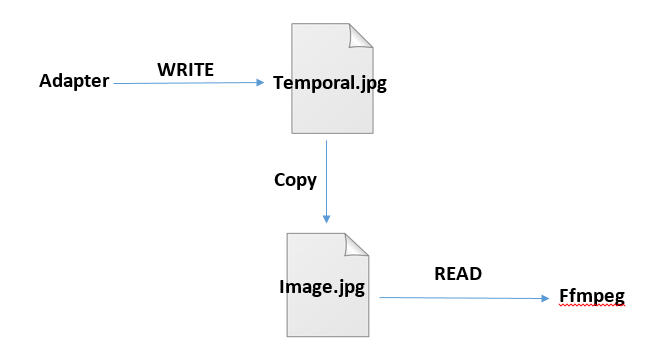
\includegraphics[width=150mm]{doblebuffer.png}
        \caption{Técnica de doble buffer}
    \end{figure}


\end{itemize}


En el adaptador finalmente se ha elegido la segunda opción debido a que es compatible con ambos codificadores. A continuación se puede observar el código mediante el cual las imágenes son obtenidas y almacenadas localmente. Cabe destacar que el adaptador presenta dos formas de ejecución, con la diferencia de que en una de ellas se despliega un interfaz en el cual se pueden observar las imágenes obtenidas de cameraserver a la frecuencia que este las envía siendo el resultado final un vídeo.
\\
\begin{lstlisting}[language=Python]

def updateImage(self):

        img = self.getCamera().getImage()
        if img is not None:
            im = Image.fromarray(img)
            im.save("temp.jpg")
            os.rename("temp.jpg","imagen.jpg")
            if self.GUI:
                showGUI(img)
                
\end{lstlisting}

Este método pertenece a la clase CameraWidget, dicha clase posee un atributo denominado camera, en la instanciación de la clase a este atributo se le asigna el valor de la cámara obtenida mediante cameraserver que a su vez implementa el método getImage que devuelve un array con los datos de la imagen que posteriormente es convertido a una imagen. 

\subsection{Aplicación web StreamingDron}

Una vez desarrollado el adaptador, se va a llevar a cabo la culminación de este objetivo. Para ello se ha desarrollado una aplicación web con el objetivo de facilitar el manejo de YouTube y sobre todo de Ffmpeg a aquellos usuarios que no sean demasiado expertos en el mundo de las retransmisiones.

Para la construcción de esta aplicación se ha reusado gran parte del código escrito anteriormente para SurveillanceApp. De esta forma la aplicación nuevamente se encuentra asociada un canal de YouTube. Para la comunicación entre YouTube y la aplicación se usan las librerías de Python pertenecientes a YouTube API, que se comunican con nuestro servidor a través del modulo child\_process usado anteriormente.

La aplicación es mas sencilla que su predecesora SurveillanceApp en cuanto al manejo de YouTube se refiere, debido a que el objetivo de manejar YouTube ya fue conseguido en dicha aplicación, por lo que se ha eliminado la parte de creación de eventos y la lista de eventos programados.

Para dar paso al desarrollo de la aplicación es necesario saber que esta se divide en dos interfaces, una pública y otra privada. Dentro de la interfaz pública se muestra la reproducción de los eventos asociados al canal que se encuentran en directo en ese momento, si es que los hubiera. Para mostrarlos se hace uso del método list tanto del recurso de liveBroadcast como de liveStream suministrándole como filtros el estado del evento que en este caso sera activo, dicho código se encuentra explicado en la sección de SurveillanceApp.

Por otro lado nos encontramos con una interfaz privada, dicha privacidad es debido a que la aplicación maneja datos sensibles relacionados con la cuenta de Google del administrador de la aplicación. De nuevo se ha reutilizado el mecanismo de seguridad de SurveillanceApp consistente en un middleware y un posterior establecimiento de sesión. Una vez superado el proceso de identificación correctamente accedemos a una interfaz en la cual podremos comenzar la retransmisión de nuestros eventos.

 
    \begin{figure}[H]
        \centering
        \includegraphics[width=150mm]{privateSD.PNG}
        \caption{Interfaz Privada}
    \end{figure}


Iniciar un evento implica la ejecución de nuestro adaptador de ffmpeg a JdeRobot así como el propio ffmpeg, para dicho trabajo se ha usado un script de python el cual genera un hilo de ejecución paralelo al principal que se encarga del adaptador mientras el hilo principal ejecuta ffmpeg.

\\
\begin{lstlisting}[language=Python]

def list_streams(path,stream_key,resolution,bitrate):
  
  command ='ffmpeg -f alsa -ac 2 -i default -f image2 -framerate 15 -loop 1 -i ' + path + ' -vcodec libx264 -preset veryfast -minrate ' + bitrate  + ' -maxrate 1000k -bufsize 1000k -vf "format=yuv420p"  -g 30 -vf drawtext="fontfile=/usr/share/fonts/truetype/freefont/FreeSerif.ttf:fontsize=24:fontcolor=yellow:textfile=./public/static/subtitles.txt:reload=1:x=100:y=50" -c:a libmp3lame -b:a 128k -ar 44100 -force_key_frames 0:00:04 -f flv rtmp://a.rtmp.youtube.com/live2/'+ stream_key
  os.system(command)
  
if __name__ == "__main__":
  try:
    subProcess = Popen(['python3','./public/JdeRobot/ffmpegAdapter/ffmpeg-adapter.py', '--Ice.Config=./public/JdeRobot/ffmpegAdapter/adapter_conf.cfg'])
    list_streams(sys.argv[1],sys.argv[2],sys.argv[3],sys.argv[4])
  except:
    print("ERROR")
    
\end{lstlisting}

Después de que ffmpeg haya comenzado la retransmisión del evento con éxito, desde el interfaz web podremos añadir subtítulos a nuestra emisión así como dar por finalizado nuestro evento, de forma que acabaremos con el proceso de ffmpeg. 

\subsection{Experimentos}

Todas estas herramientas han sido desarrolladas con el objetivo final de ejecutarlas junto con un UAV real por ello una vez desarrollados todos los componentes se pasa a la fase de experimentación. Esta fase a su vez se divide en dos partes la simulación y la prueba real.

Debido a que los UAV son aparatos costosos no se puede experimentar con ellos directamente sin antes pasar por un periodo de simulación, de dicha simulación se encargara Gazebo del que ya hablamos en el capitulo de introducción. Actualmente disponemos de distintos escenarios de simulación compatibles con JdeRobot.Además de Gazebo nos apoyaremos en UAViewer para teleoperar el Dron.Los escenarios de Gazebo simulan  un UAV que posee los cuatro interfaces que manejamos en JdeRobot proporcionados por el arDroneServer(todas estas herramientas están explicadas en el capitulo 3), para nuestro adaptador únicamente necesitamos la interfaz Camera pero para el manejo del Dron si necesitaremos los demás interfaces.

  \begin{figure}[H]
        \centering
        \includegraphics[width=150mm]{expGazebo.PNG}
        \caption{Arquitectura Experimento}
    \end{figure}

Para conectar Gazebo con nuestro adaptador y poder recuperar las imágenes proporcionadas por la cámara, únicamente se debe configurar el fichero "adapter\_conf.cfg", con la ip y el puerto correcto donde Gazebo se esta ejecutando, una vez conectado a través de ffmpeg, OBS o la aplicación web se comienza la retransmisión hacia Youtube del contenido captado por el UAV.
La ejecución de este experimento puede verse en la wiki oficial del proyecto \footnote{http://jderobot.org/Apavo-tfg#YouTube_.26_JdeRobot}

\subsubsection{Experimentos con Drone real}

Una vez testeada con éxito la aplicación en un entorno simulado se puede proceder a realizar las pruebas con el drone real.Para el experimento usaremos el modelo Ar Drone fabricado por la marca Parrot y proporcionado por el equipo de robótica de la URJC, dicho dron es un cuadricoptero totalmente compatible con las herramientas de JdeRobot.

  \begin{figure}[H]
        \centering
        \includegraphics[width=150mm]{arDrone.png}
        \caption{arDrone de Parrot}
    \end{figure}

Para realizar las pruebas nos apoyaremos en el arDrone server como forma de conexión con el aparato y en UAViewer para el manejo del dron.Por otro lado para nuestro adaptador y posterior comunicación con YouTube únicamente recuperaremos el interfaz de la cámara, como en el experimento del simulador.

ArDrone server posee un fichero de configuración que podemos ver a continuación, en el se encuentran detallados en que dirección ip y puerto se esta recibiendo información de cada uno de los interfaces así como los nombre que toman estos.

\begin{lstlisting}

ArDrone.Camera.Endpoints=default -h 0.0.0.0 -p 9999
ArDrone.Camera.Name=ardrone_camera
ArDrone.Camera.FramerateN=15
ArDrone.Camera.FramerateD=1
ArDrone.Camera.Format=RGB8
ArDrone.Camera.ArDrone2.ImageWidth=640
ArDrone.Camera.ArDrone2.ImageHeight=360
ArDrone.Camera.ArDrone1.ImageWidth=320
ArDrone.Camera.ArDrone1.ImageHeight=240
# If you want a mirror image, set to 1
ArDrone.Camera.Mirror=0


ArDrone.Pose3D.Endpoints=default -h 0.0.0.0 -p 9998
ArDrone.Pose3D.Name=ardrone_pose3d

ArDrone.RemoteConfig.Endpoints=default -h 0.0.0.0 -p 9997
ArDrone.RemoteConfig.Name=ardrone_remoteConfig

ArDrone.Navdata.Endpoints=default -h 0.0.0.0 -p 9996
ArDrone.Navdata.Name=ardrone_navdata

ArDrone.CMDVel.Endpoints=default -h 0.0.0.0 -p 9995
ArDrone.CMDVel.Name=ardrone_cmdvel

ArDrone.Extra.Endpoints=default -h 0.0.0.0 -p 9994
ArDrone.Extra.Name=ardrone_extra

ArDrone.NavdataGPS.Endpoints=default -h 0.0.0.0 -p 9993
ArDrone.NavdataGPS.Name=ardrone_navdatagps

\end{lstlisting}

Tanto para conectar UAViewer como nuestro adaptador a arDroneServer necesitamos editar los ficheros de configuración de forma que las ips, puertos y nombres de los interfaces de los que deseamos recuperar información coincidan. A continuación podemos ver la configuración del adaptador para poder recuperar imagenes de la camara.

\begin{lstlisting}
Introrob.Camera.Proxy  = ardrone_camera:default -h 0.0.0.0 -p 9999
\end{lstlisting}

En la realización del experimento nos encontramos con un problema de red no previsto antes. Dicho problema consiste en que el dron crea una red wifi a la cual debemos conectar nuestro PC para poder comunicarnos con él a través de las herramientas desarrolladas, el problema es que dicha red no presenta conexión a internet por lo cual aunque la conexión con el dron es satisfactoria la comunicación con YouTube no se puede llevar a cabo ya que requiere de conexión a internet.

La solución a este problema es crear dentro del mismo PC dos conexiones de red, una conexión wifi para interactuar con el dron y la otra conexión vía ethernet con acceso a internet.

\begin{figure}[H]
        \centering
        \includegraphics[width=150mm]{realDroneArq.png}
        \caption{Arquitectura Experimento}
    \end{figure}

Debido a que JdeRobot se ejecuta bajo el sistema operativo Linux, para conseguir esta configuración de red hemos accedido manualmente a la configuración de red del sistema aportado una dirección pública vía ethernet suministrada por la universidad en la que levantaremos el servidor nodejs de la aplicación mientras que en la segunda red estableceremos una conexión vía wifi con el UAV. 

Una vez realizadas todas las conexiones el experimento se ha llevado a cabo con éxito, este experimento puede verse al completo en la wiki oficial del proyecto \footnote{http://jderobot.org/Apavo-tfg#Fly_with_Real_Drone}

